\subsection{Testing transmission}
This are the results for the CRC correction seen on Arduino console.


\begin{figure}[!htbp]
	\centering
	\begin{tabular}{cc}
		\begin{subfigure}{.2\textwidth}
			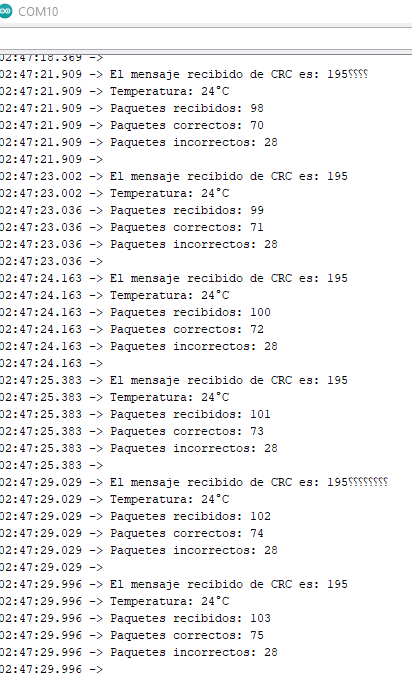
\includegraphics[width=2cm]{images/10cm_p1.png}
			\subcaption{Testing P=1001.}
		\end{subfigure} &
		\begin{subfigure}{.2\textwidth}
			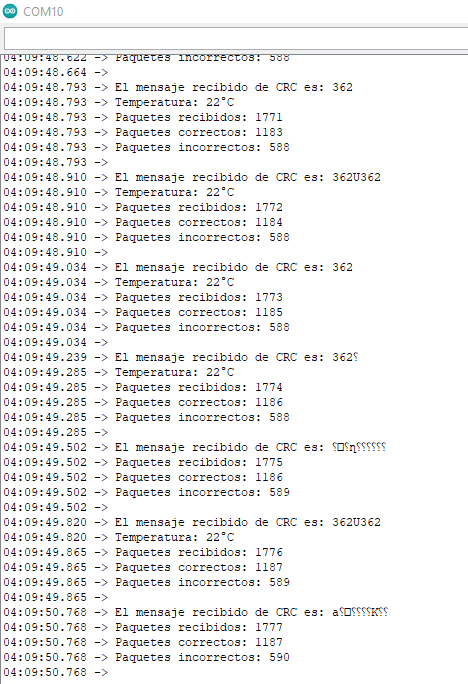
\includegraphics[width=2cm]{images/10cm_p2.png}
			\subcaption{Testing P=11001}
		\end{subfigure}
	\end{tabular}
	\caption{Distance 10cm}
\end{figure}

\newpage
\begin{figure}  [!htbp]
	\centering
	\begin{tabular}{cc}
			\begin{subfigure}{.2\textwidth}
				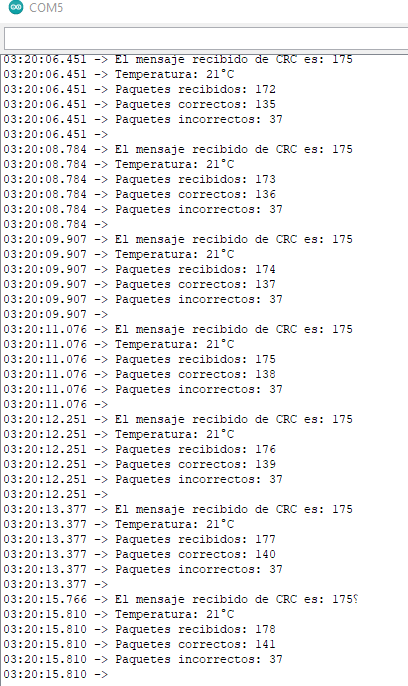
\includegraphics[width=3cm]{images/50cm_p1.png}
				\subcaption{Testing P=1001.}
			\end{subfigure} &
			\begin{subfigure}{.2\textwidth}
				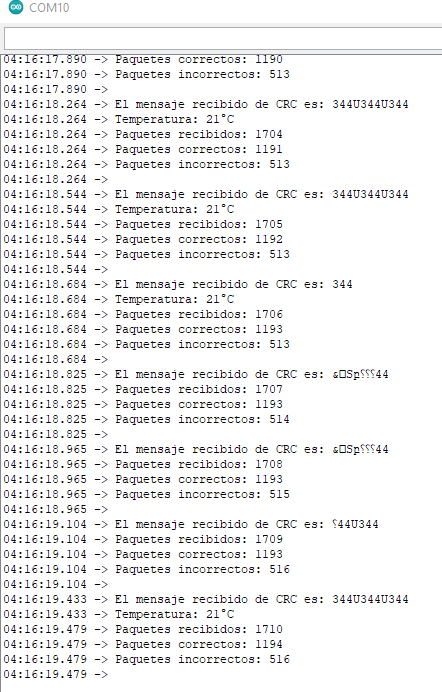
\includegraphics[width=3cm]{images/50cm_p2.png}
				\subcaption{Testing P=11001}
			\end{subfigure}
	\end{tabular}
	\caption{Distance 50cm}
\end{figure}

\begin{figure}[!htbp]
	\centering
	\begin{tabular}{cc}
		\begin{subfigure}{.2\textwidth}
			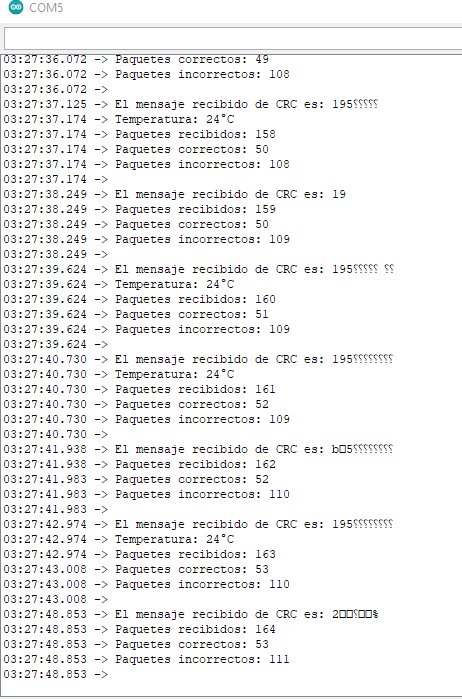
\includegraphics[width=3cm]{images/1m_p1.png}
			\subcaption{Testing P=1001.}
		\end{subfigure} &
		\begin{subfigure}{.2\textwidth}
			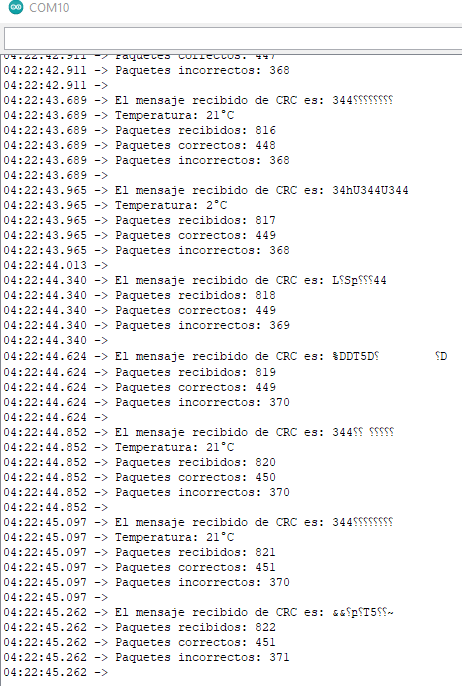
\includegraphics[width=3cm]{images/1m_p2.png}
			\subcaption{Testing P=11001}
		\end{subfigure}
	\end{tabular}
	\caption{Distance 1m}
\end{figure}

\begin{figure}[!htbp]
	\centering
	\begin{tabular}{cc}
		\begin{subfigure}{.2\textwidth}
			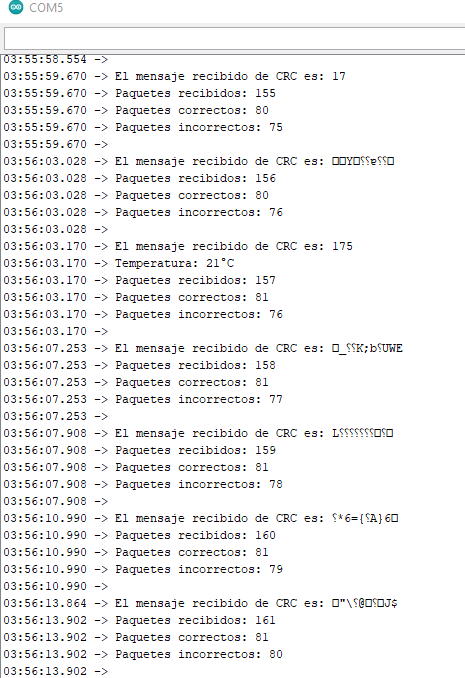
\includegraphics[width=3cm]{images/5m_p1.png}
			\subcaption{Testing P=1001.}
		\end{subfigure} &
		\begin{subfigure}{.2\textwidth}
			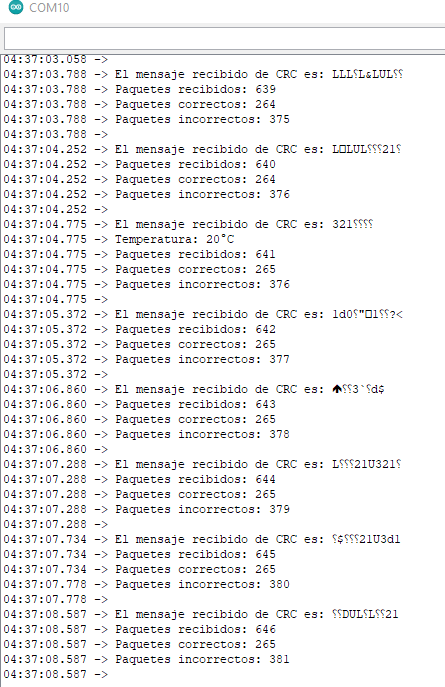
\includegraphics[width=3cm]{images/5m_p2.png}
			\subcaption{Testing P=11001}
		\end{subfigure}
	\end{tabular}
	\caption{Distance 5m}
\end{figure}

\newpage
\begin{figure}[!htbp]
	\centering
	\begin{tabular}{cc}
		\begin{subfigure}{.2\textwidth}
			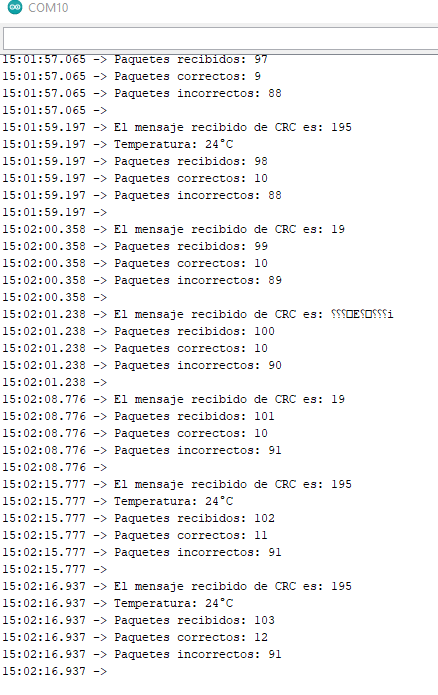
\includegraphics[width=3cm]{images/10m_p1.png}
			\subcaption{Testing P=1001.}
		\end{subfigure} &
		\begin{subfigure}{.2\textwidth}
			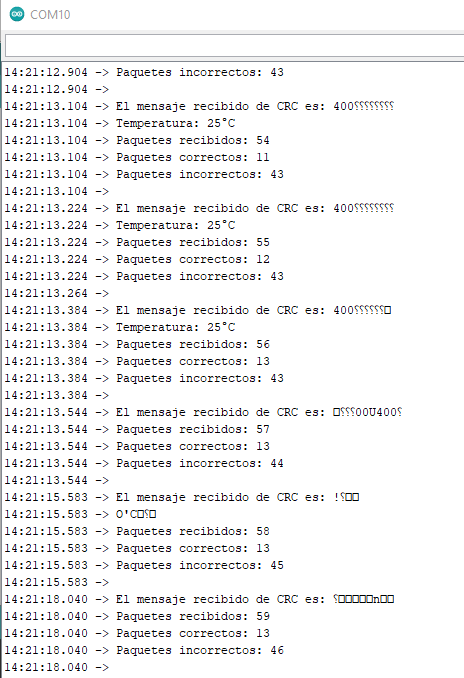
\includegraphics[width=3cm]{images/10m_p2.png}
			\subcaption{Testing P=11001}
		\end{subfigure}
	\end{tabular}
	\caption{Distance 10m}
\end{figure}

\begin{figure}[!htbp]
	\centering
	\begin{tabular}{cc}
		\begin{subfigure}{.2\textwidth}
			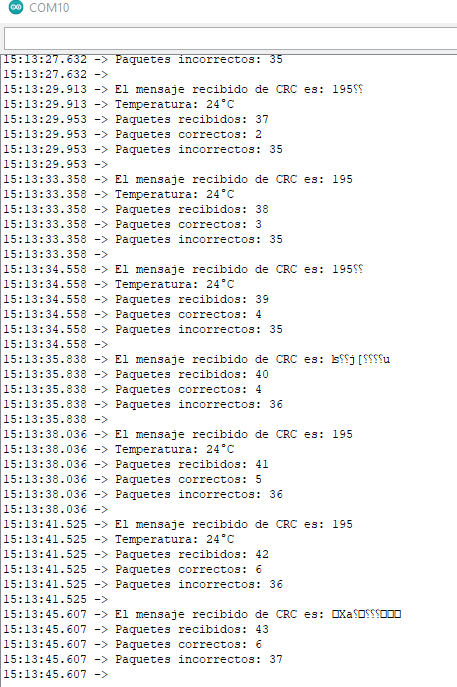
\includegraphics[width=3cm]{images/15m_p1.png}
			\subcaption{Testing P=1001.}
		\end{subfigure} &
		\begin{subfigure}{.2\textwidth}
			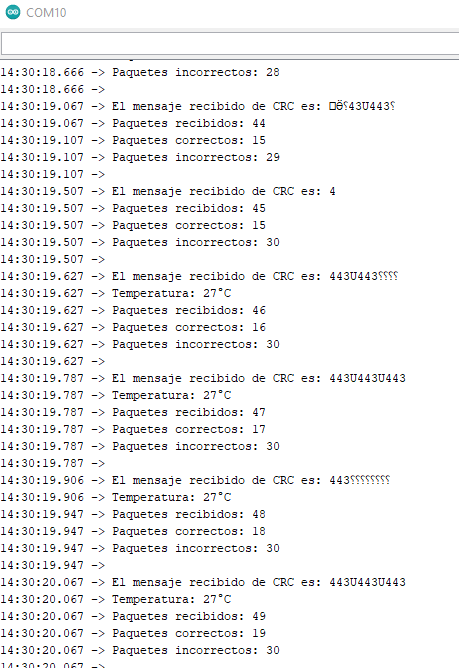
\includegraphics[width=3cm]{images/15m_p2.png}
			\subcaption{Testing P=11001}
		\end{subfigure}
	\end{tabular}
	\caption{Distance 15m}
\end{figure}

\begin{figure} [!htbp]
	\centering
	\begin{tabular}{cc}
		\begin{subfigure}{.2\textwidth}
			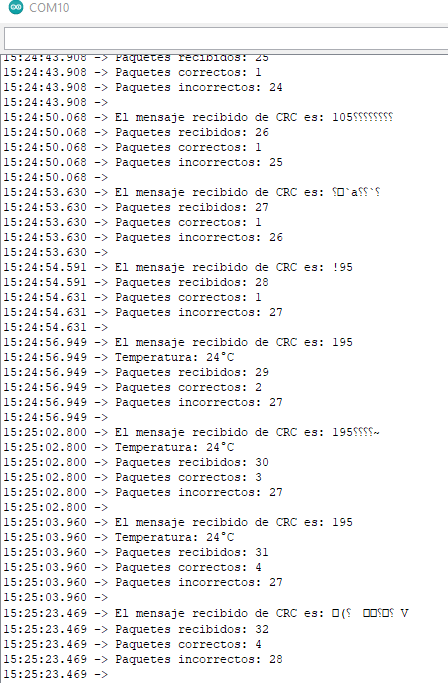
\includegraphics[width=3cm]{images/20m_p1.png}
			\subcaption{Testing P=1001.}
		\end{subfigure} &
		\begin{subfigure}{.2\textwidth}
			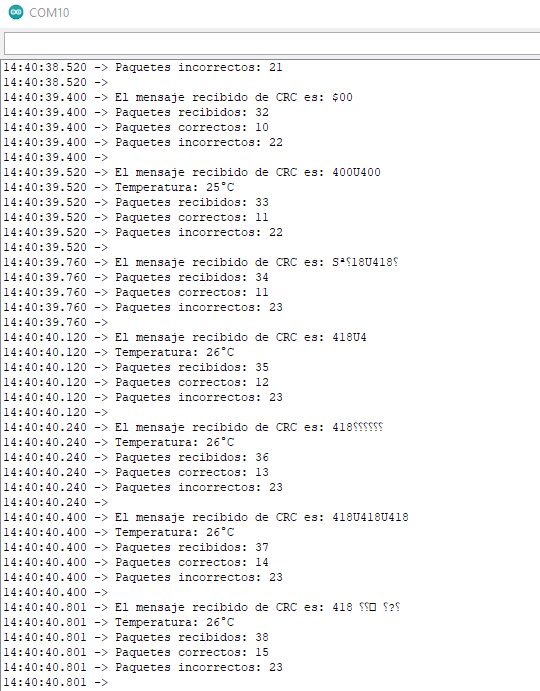
\includegraphics[width=3cm]{images/20m_p2.png}
			\subcaption{Testing P=11001}
		\end{subfigure}
	\end{tabular}
	\caption{Distance 20m}
\end{figure}
